The goodness of the fit (GOF) indicates how well the model PDF (probability
distribution function) agrees with the data. There are various algorithms to 
compute the GOF such as {\bf{saturated}} (Baker-Cousins)~\cite{Baker:1983tu}, KS
(Kolmogorov-Smirnov)~\cite{ks1},~\cite{smirnov1948}, and 
AD (Anderson-Darling)~\cite{anderson1952}. The saturated algorithm is used in this analysis
for GOF. The test statistics as a measure of GOF is given as \cite{Baker:1983tu}
\begin{equation}
q_{\rm{GoF, saturated}} = -2\ln \left(\frac{L_{\rm{nominal}} (n|\mu s(\theta) + b(\theta))}{L_{\rm{saturated}}(n|n)}\right)
\label{eq:gof}
\end{equation}

The likelihood functions of Equation (\ref{eq:gof}) are given by
\begin{equation}
L_{\rm{nominal}} (n|\mu s(\theta) + b(\theta)) = \prod_{j=1}^N \frac{(\mu s_j(\theta) + b_j(\theta))^{n_j}}{n_{j}!} \exp(-(\mu s_j(\theta) + b_j(\theta)))
\label{eq:lNominal}
\end{equation}
and,
\begin{equation}
L_{\rm{saturated}} (n|n) = \prod_{j=1}^N \frac{(n_j)^{n_j}}{n_{j}!} \exp(-n_j)
\label{eq:lSaturated}
\end{equation}


where $n_j$ is the expectation value in $j^{\rm{th}}$ bin of data, N is the total number of bins. The
$s_j(\theta)$ and $b_j(\theta)$ are the mean number of events in $j^{\rm{th}}$ bin of signal and background
process and depend on the nuisance parameters ($\theta$). The $\mu$ is the signal strength which is
zero for background only hypothesis and non-zero for signal+background hypothesis. In $j^{\rm{th}}$ 
bin, $s_j(\theta)$ and $b_j(\theta)$ are given by \cite{Cowan:2010js}

\begin{equation}
s_{j}(\theta) = s_{\rm{tot}}\int_{j^{\rm{th}} bin} f_s(x; \theta_s)dx,
\end{equation}

\begin{equation}
b_{j}(\theta) = b_{\rm{tot}}\int_{j^{\rm{th}} bin} f_b(x; \theta_b)dx.
\end{equation}
The $f_s(x; \theta_s)$ and $f_b(x; \theta_b)$ are PDFs for signal and background events. The 
$s_{\rm{tot}}$ and $b_{\rm{tot}}$ are mean of total number of events from signal and background 
process. Using Equation (\ref{eq:lNominal}) and (\ref{eq:lSaturated}),
\begin{equation}
q_{\rm{GoF, saturated}} = 2\sum_{j}\left(\mu s_j(\theta) + b_j(\theta) - n_j + n_j\ln\left(\frac{n_j}{\mu s_j(\theta) + b_j(\theta)}\right)\right)
\label{eq:gofFinal}
\end{equation}

The goodness of fit ($q_{\rm{GoF, saturated}}$) is shown in Figure~\ref{fig:GOF} for \ljets channel  
from exclusive charm categories for all signal mass points using observed data and generated toys. 
Lower the value of GOF, the better is the agreement between data and model PDF. For different 
channels and various event categories, the values of GOF for every category, all the mass of the 
charged Higgs, and all channels are shown in Tables~\ref{tab:gofMu},~\ref{tab:gofEle}, and 
\ref{tab:gofLep}. If one normaizes Figure~\ref{fig:GOF}, then the area on the right hand side of 
the arrow (observed value of GOF) will correspond to the p-value.
\begin{figure}
    \centering  
    \subfigure[]{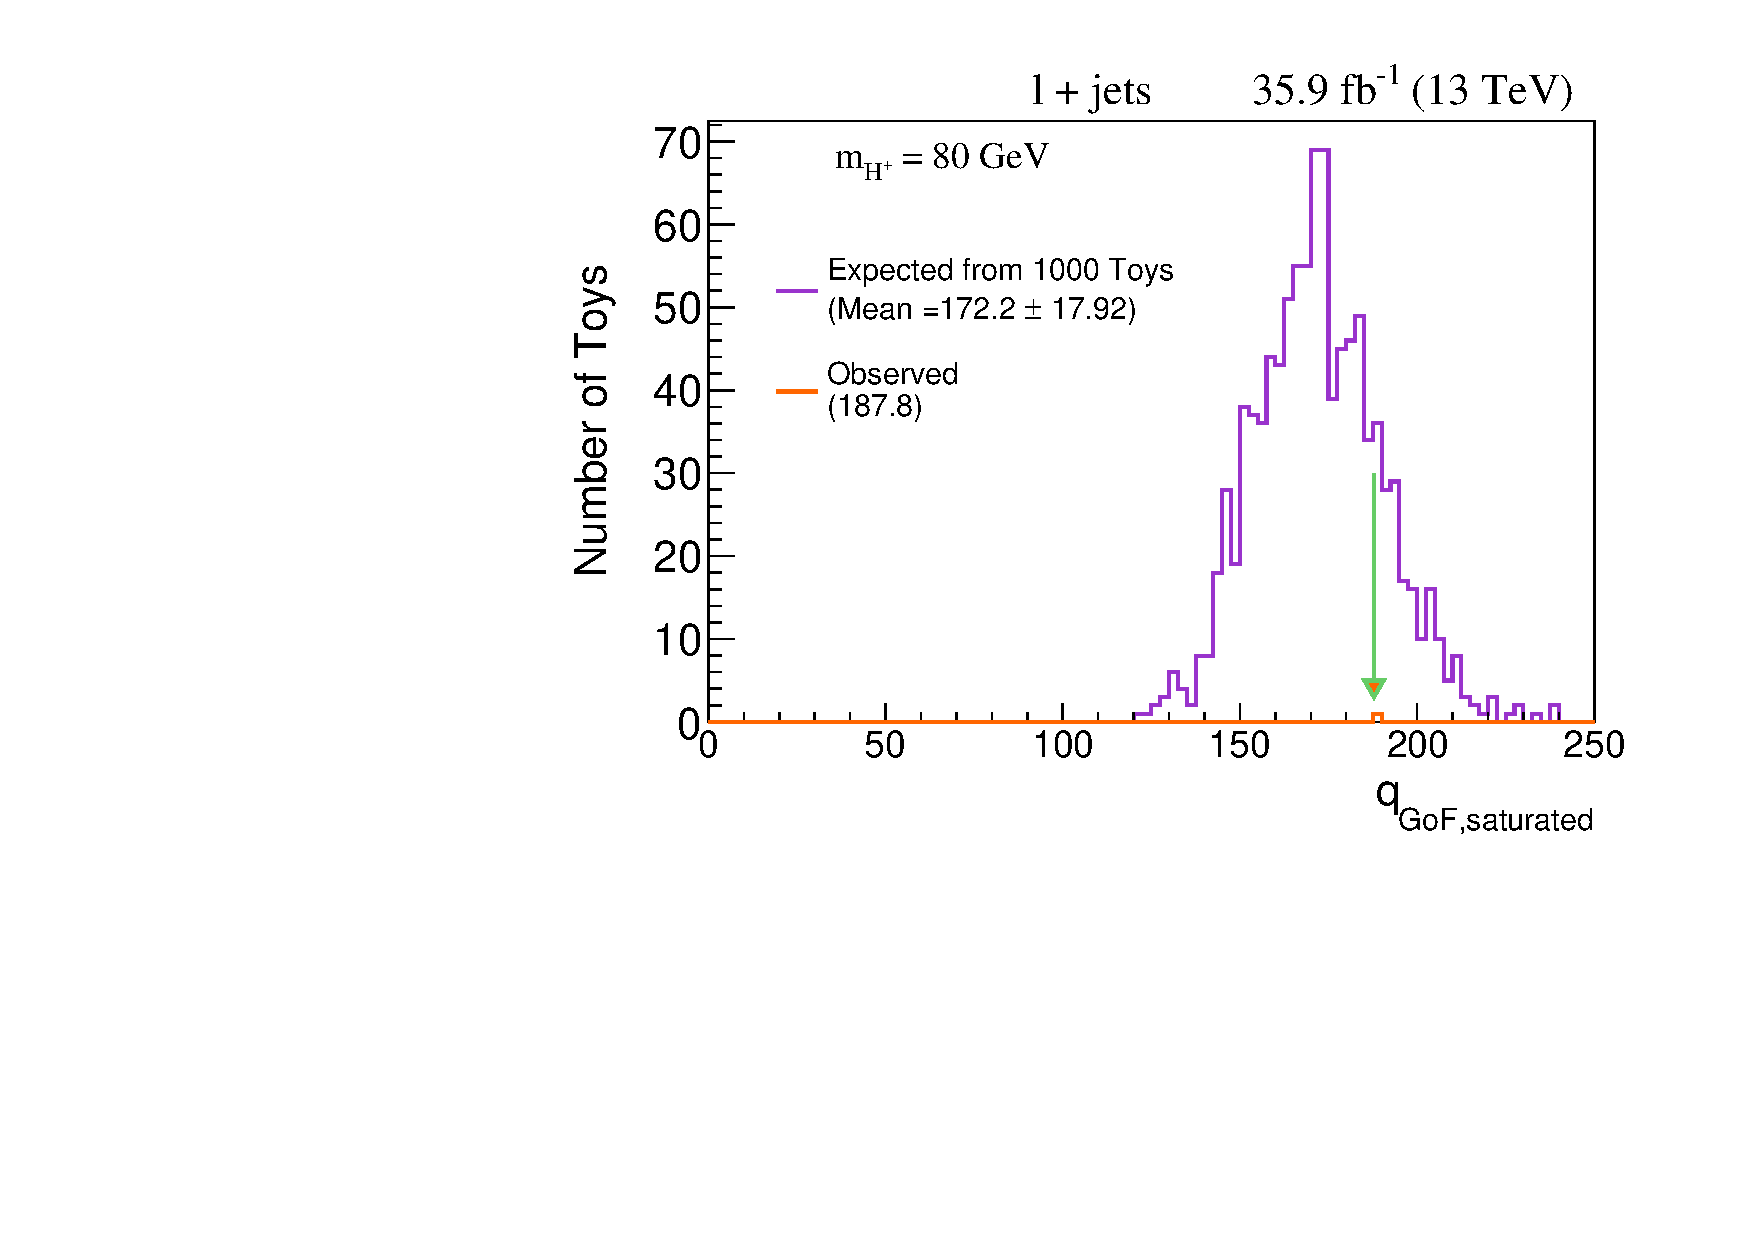
\includegraphics[width=0.40\linewidth]{Image/GOF/GOF_mu_ele_Cat3_cTagEx_80.pdf}}
    \subfigure[]{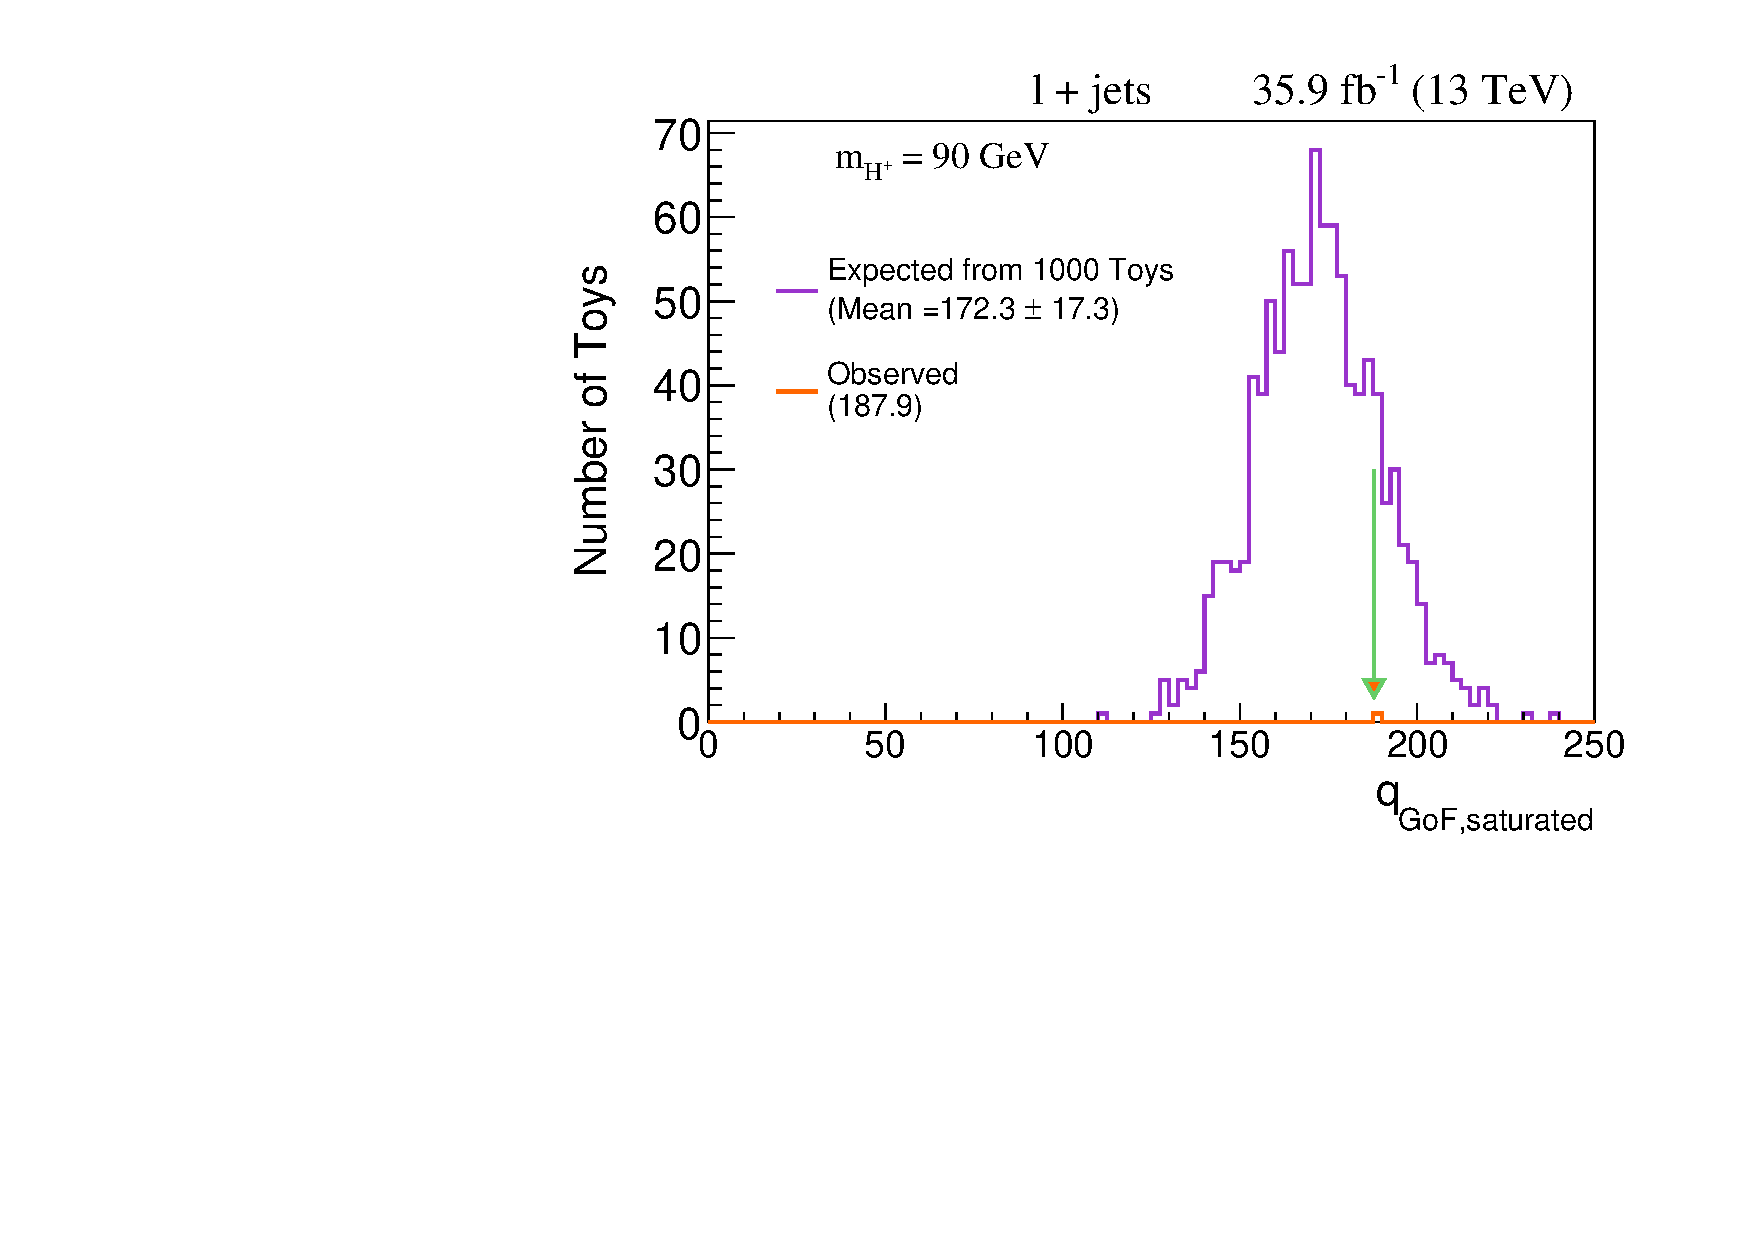
\includegraphics[width=0.40\linewidth]{Image/GOF/GOF_mu_ele_Cat3_cTagEx_90.pdf}}
    \vfil
    \subfigure[]{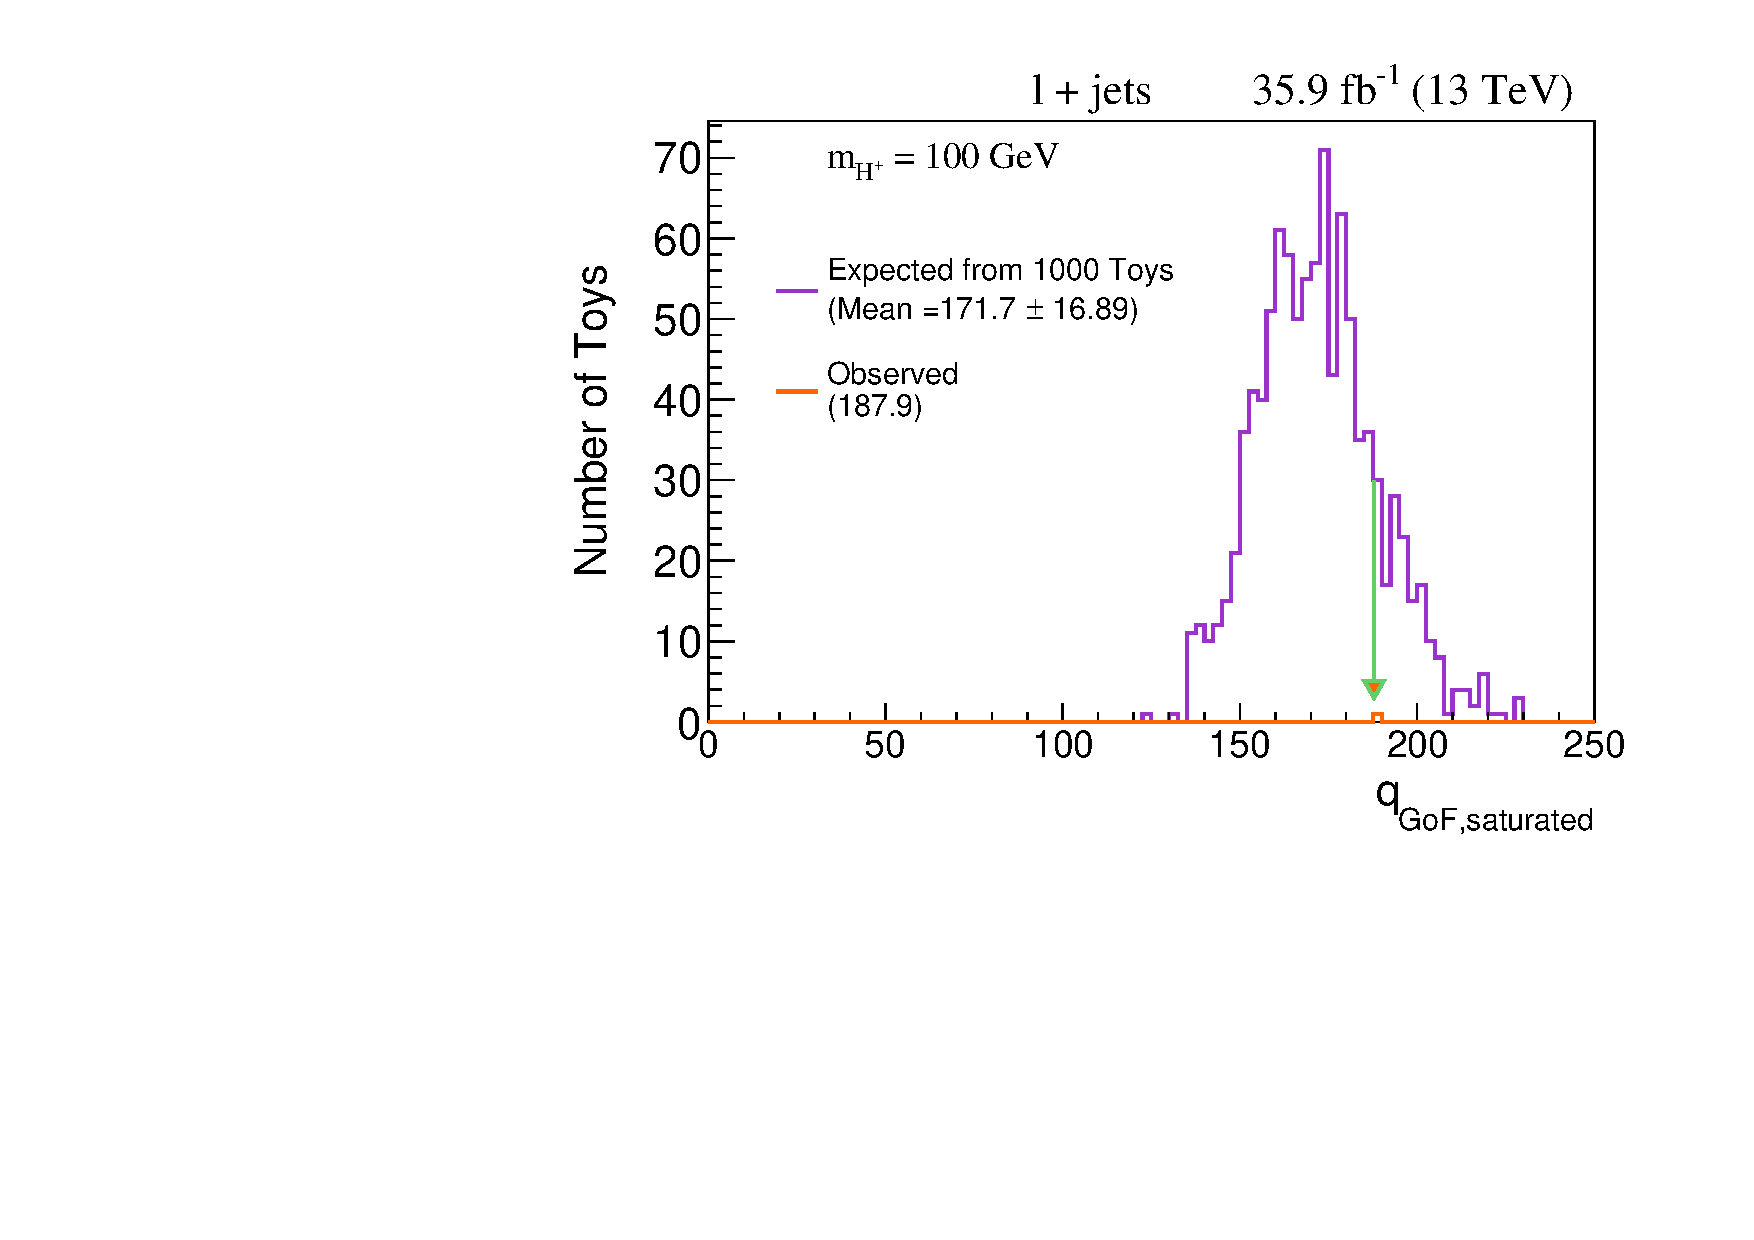
\includegraphics[width=0.40\linewidth]{Image/GOF/GOF_mu_ele_Cat3_cTagEx_100.pdf}}
    \subfigure[]{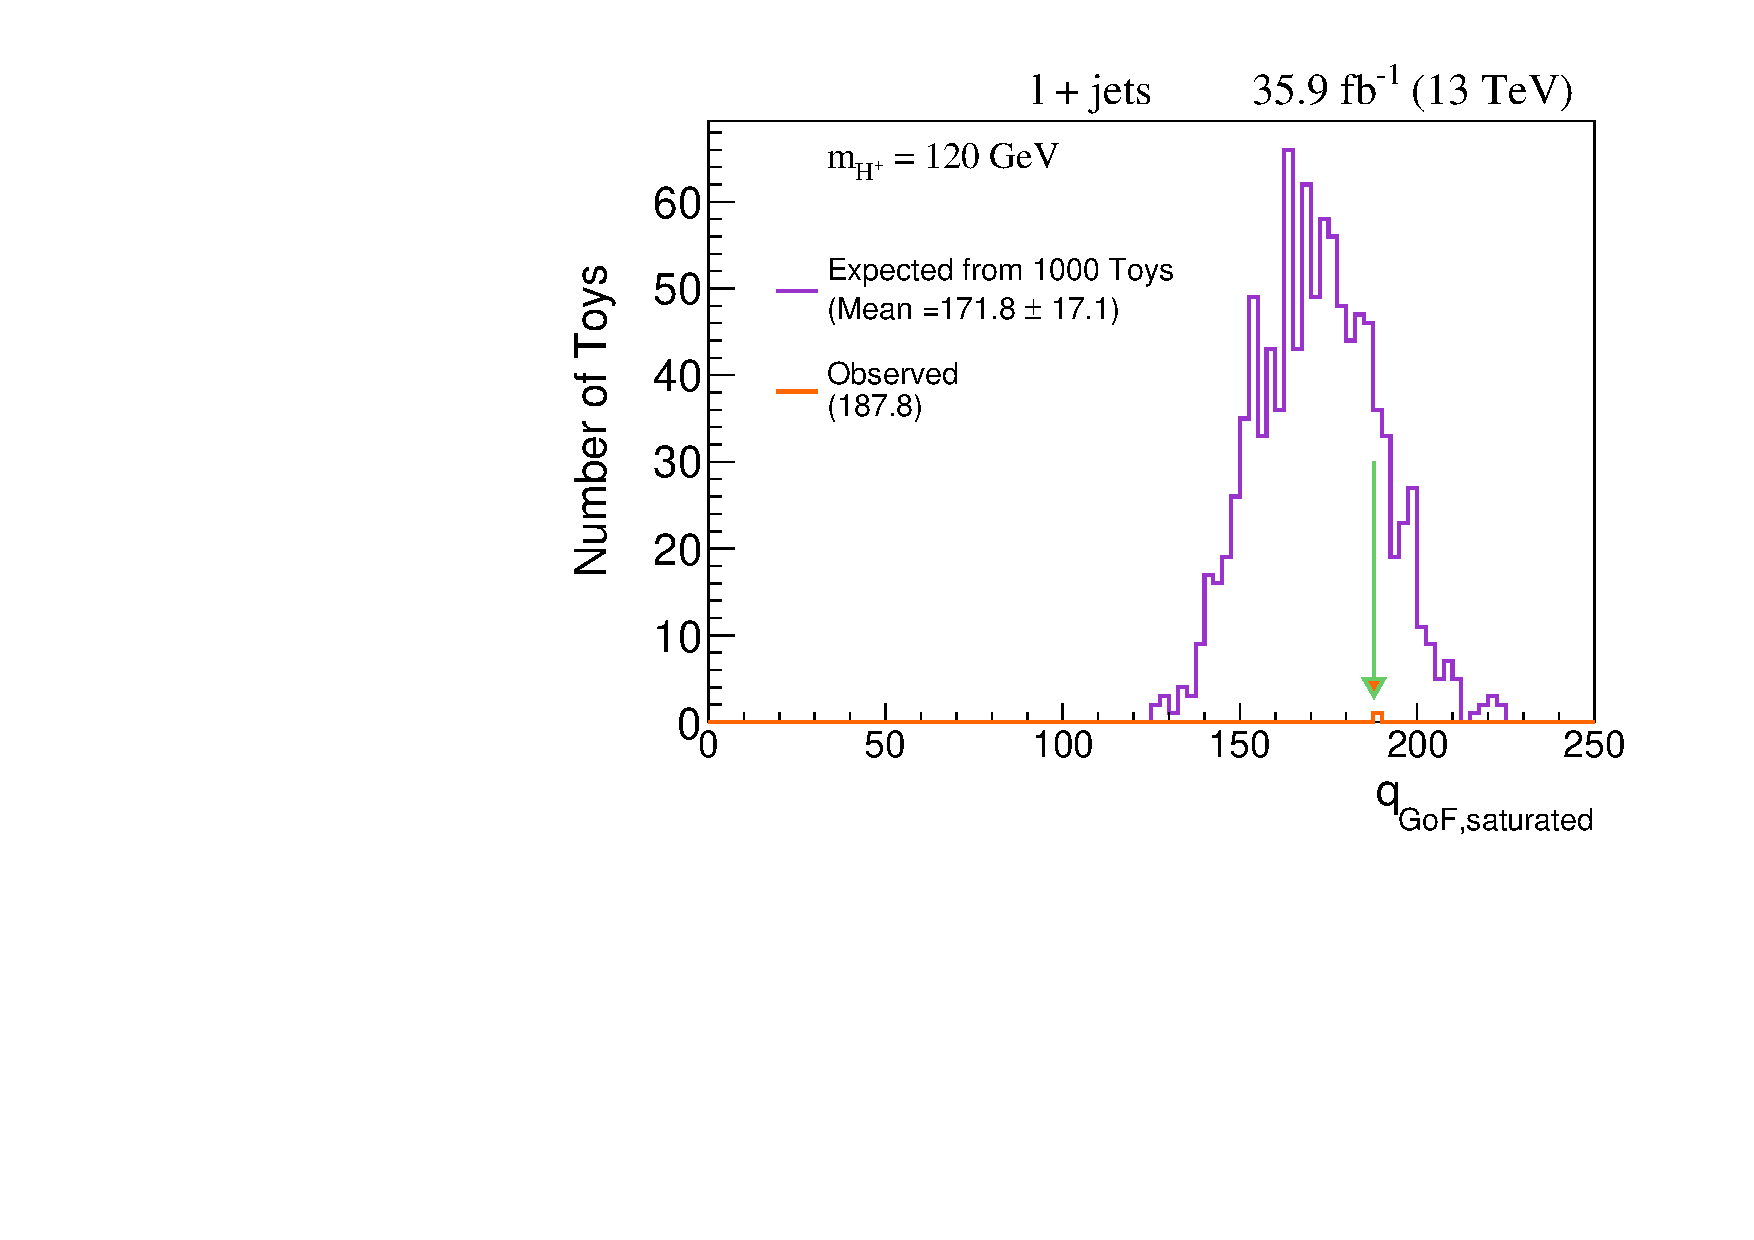
\includegraphics[width=0.40\linewidth]{Image/GOF/GOF_mu_ele_Cat3_cTagEx_120.pdf}}
    \vfil
    \subfigure[]{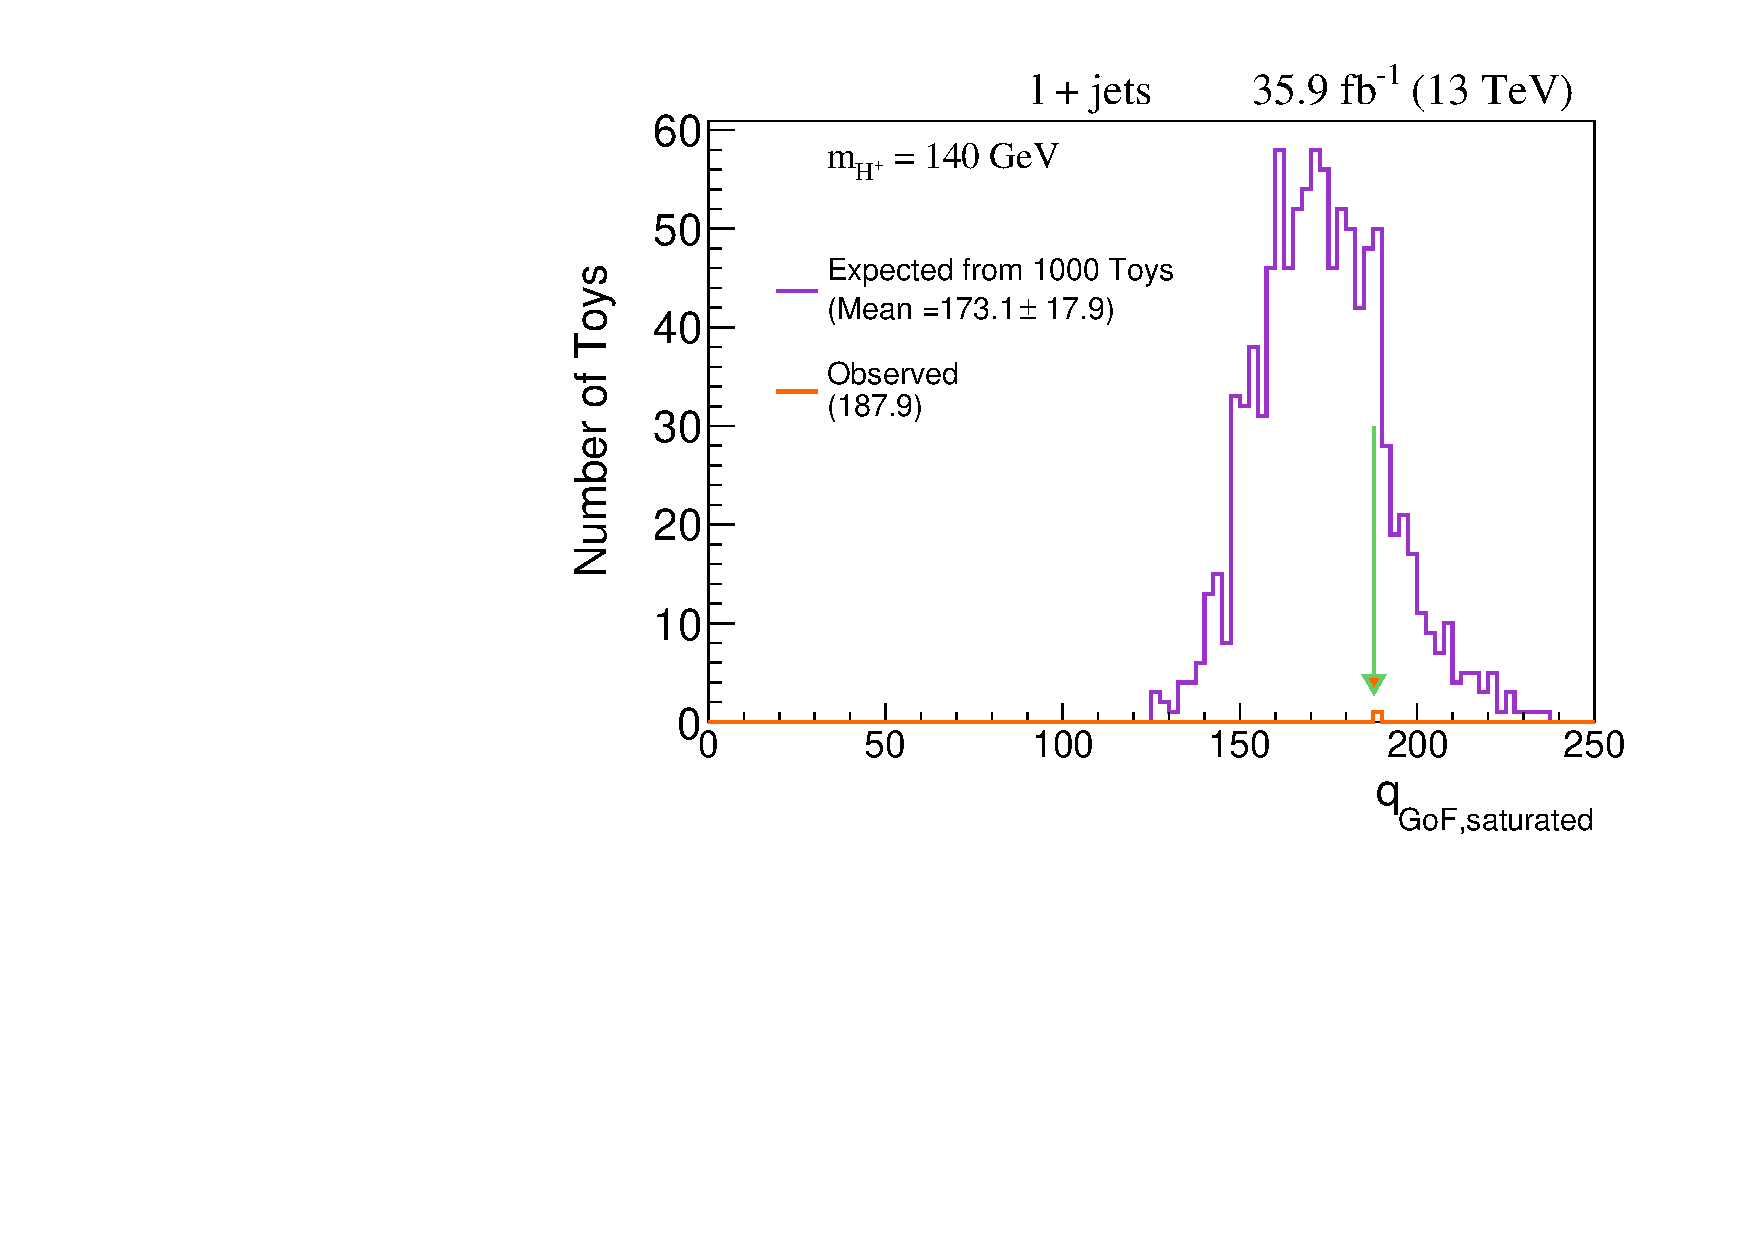
\includegraphics[width=0.40\linewidth]{Image/GOF/GOF_mu_ele_Cat3_cTagEx_140.pdf}}
    \subfigure[]{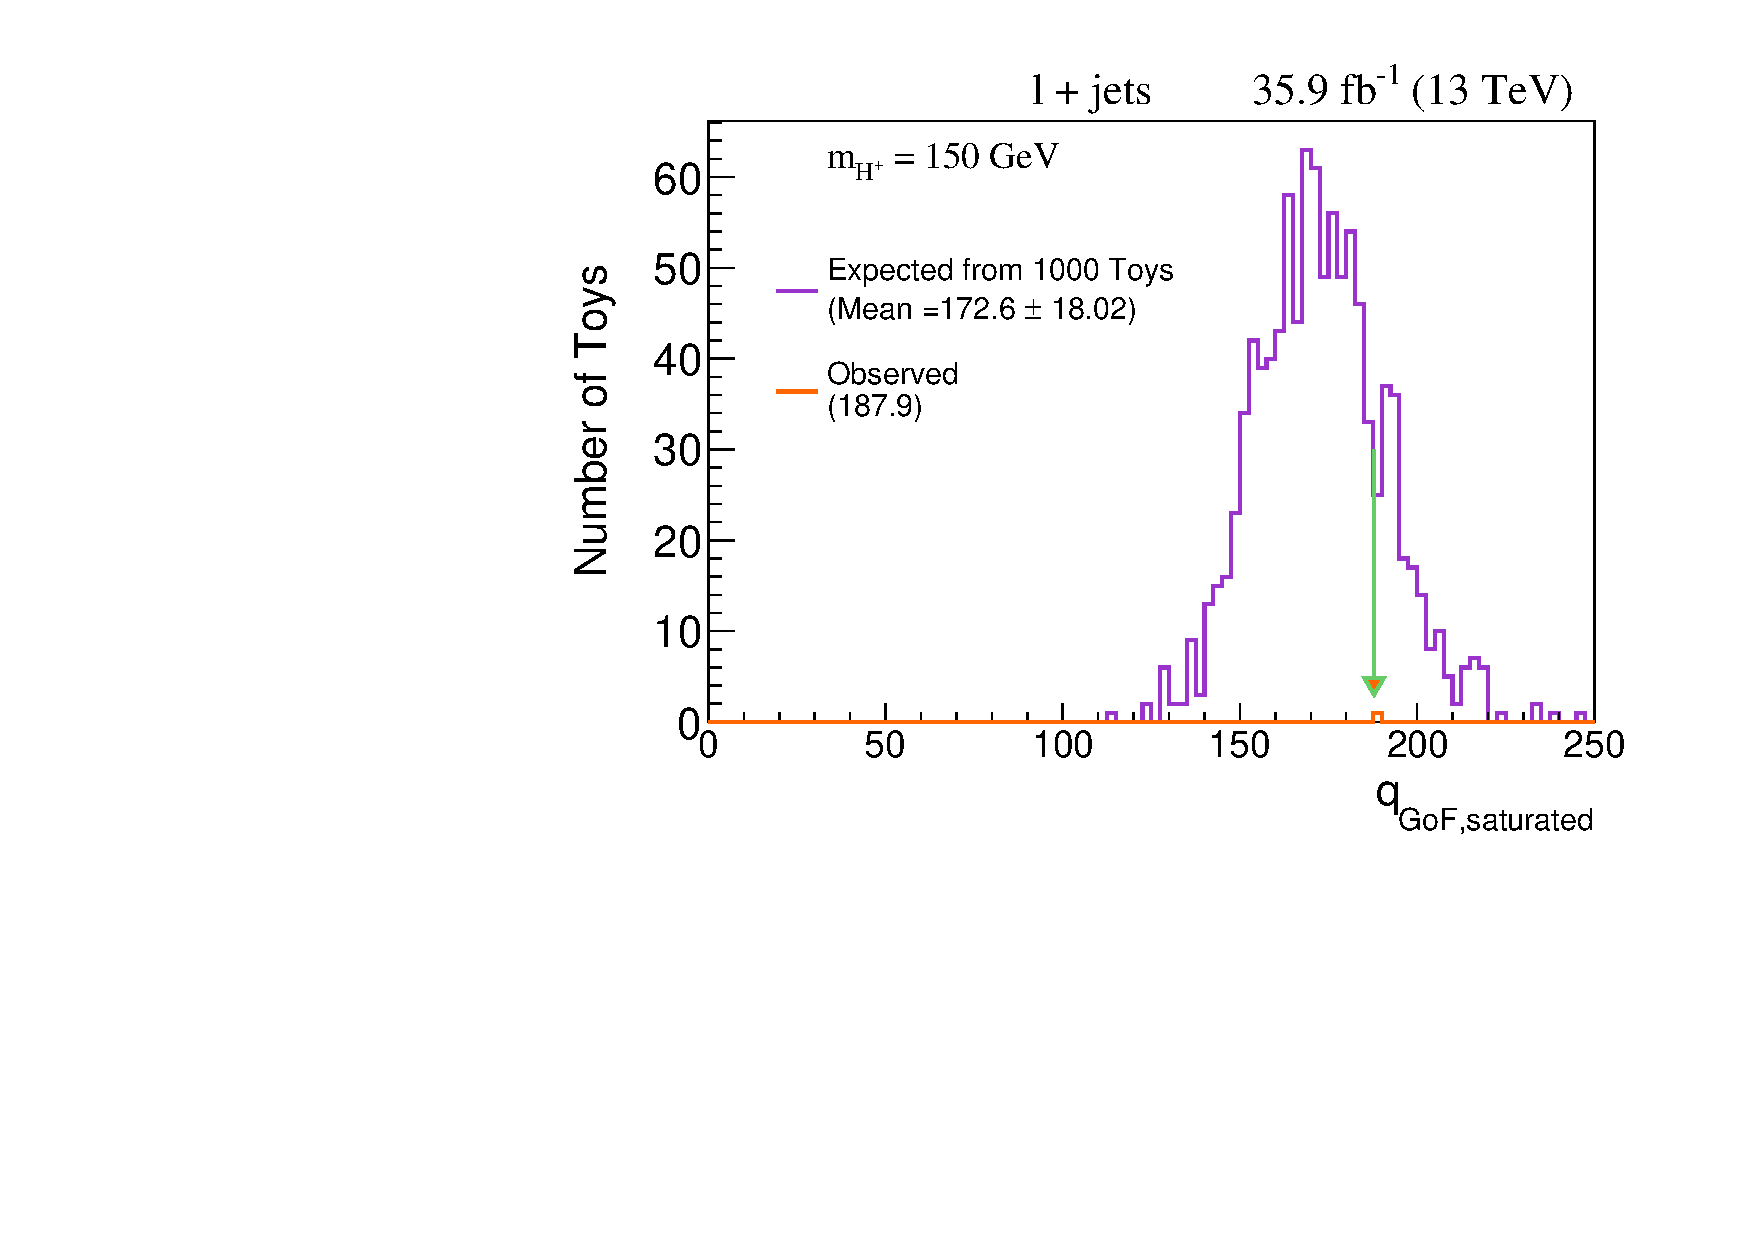
\includegraphics[width=0.40\linewidth]{Image/GOF/GOF_mu_ele_Cat3_cTagEx_150.pdf}}
    \vfil
    \subfigure[]{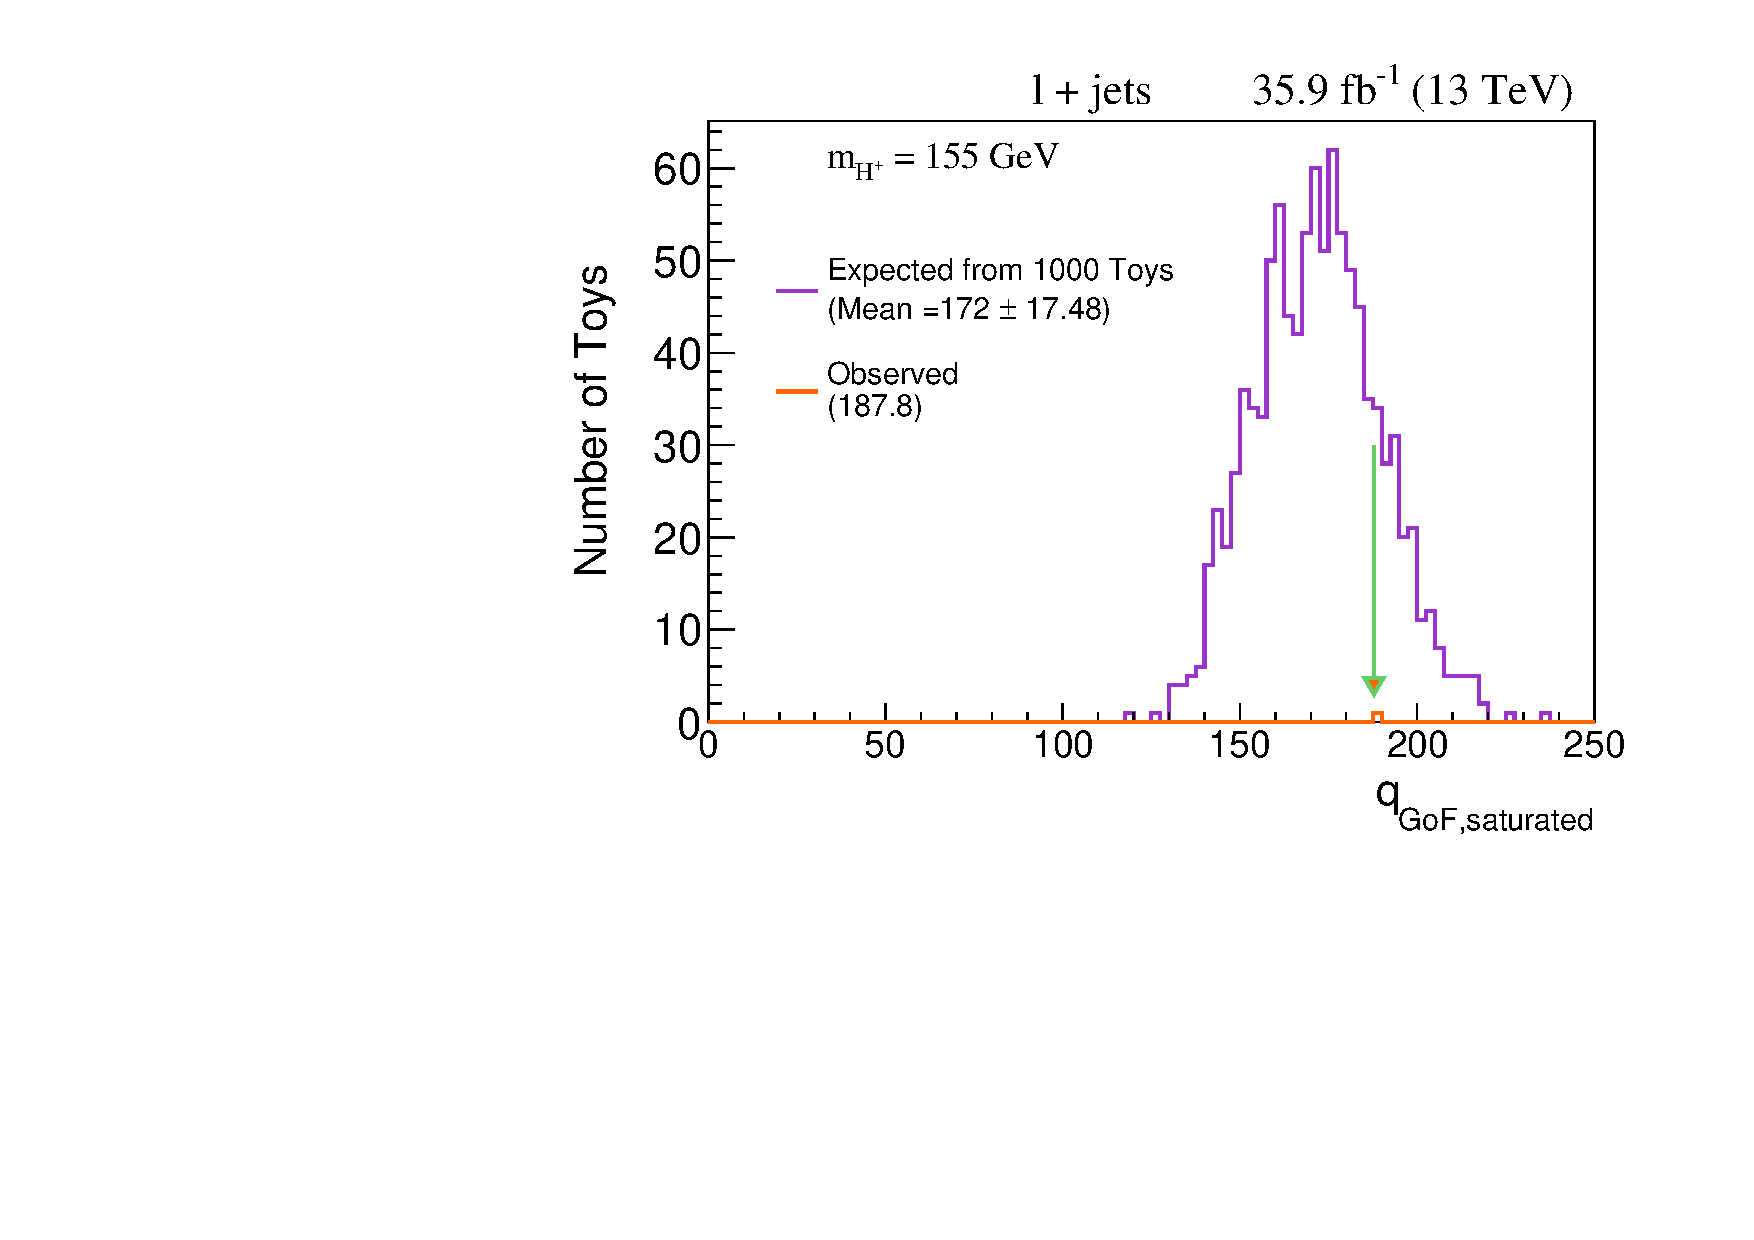
\includegraphics[width=0.40\linewidth]{Image/GOF/GOF_mu_ele_Cat3_cTagEx_155.pdf}}
    \subfigure[]{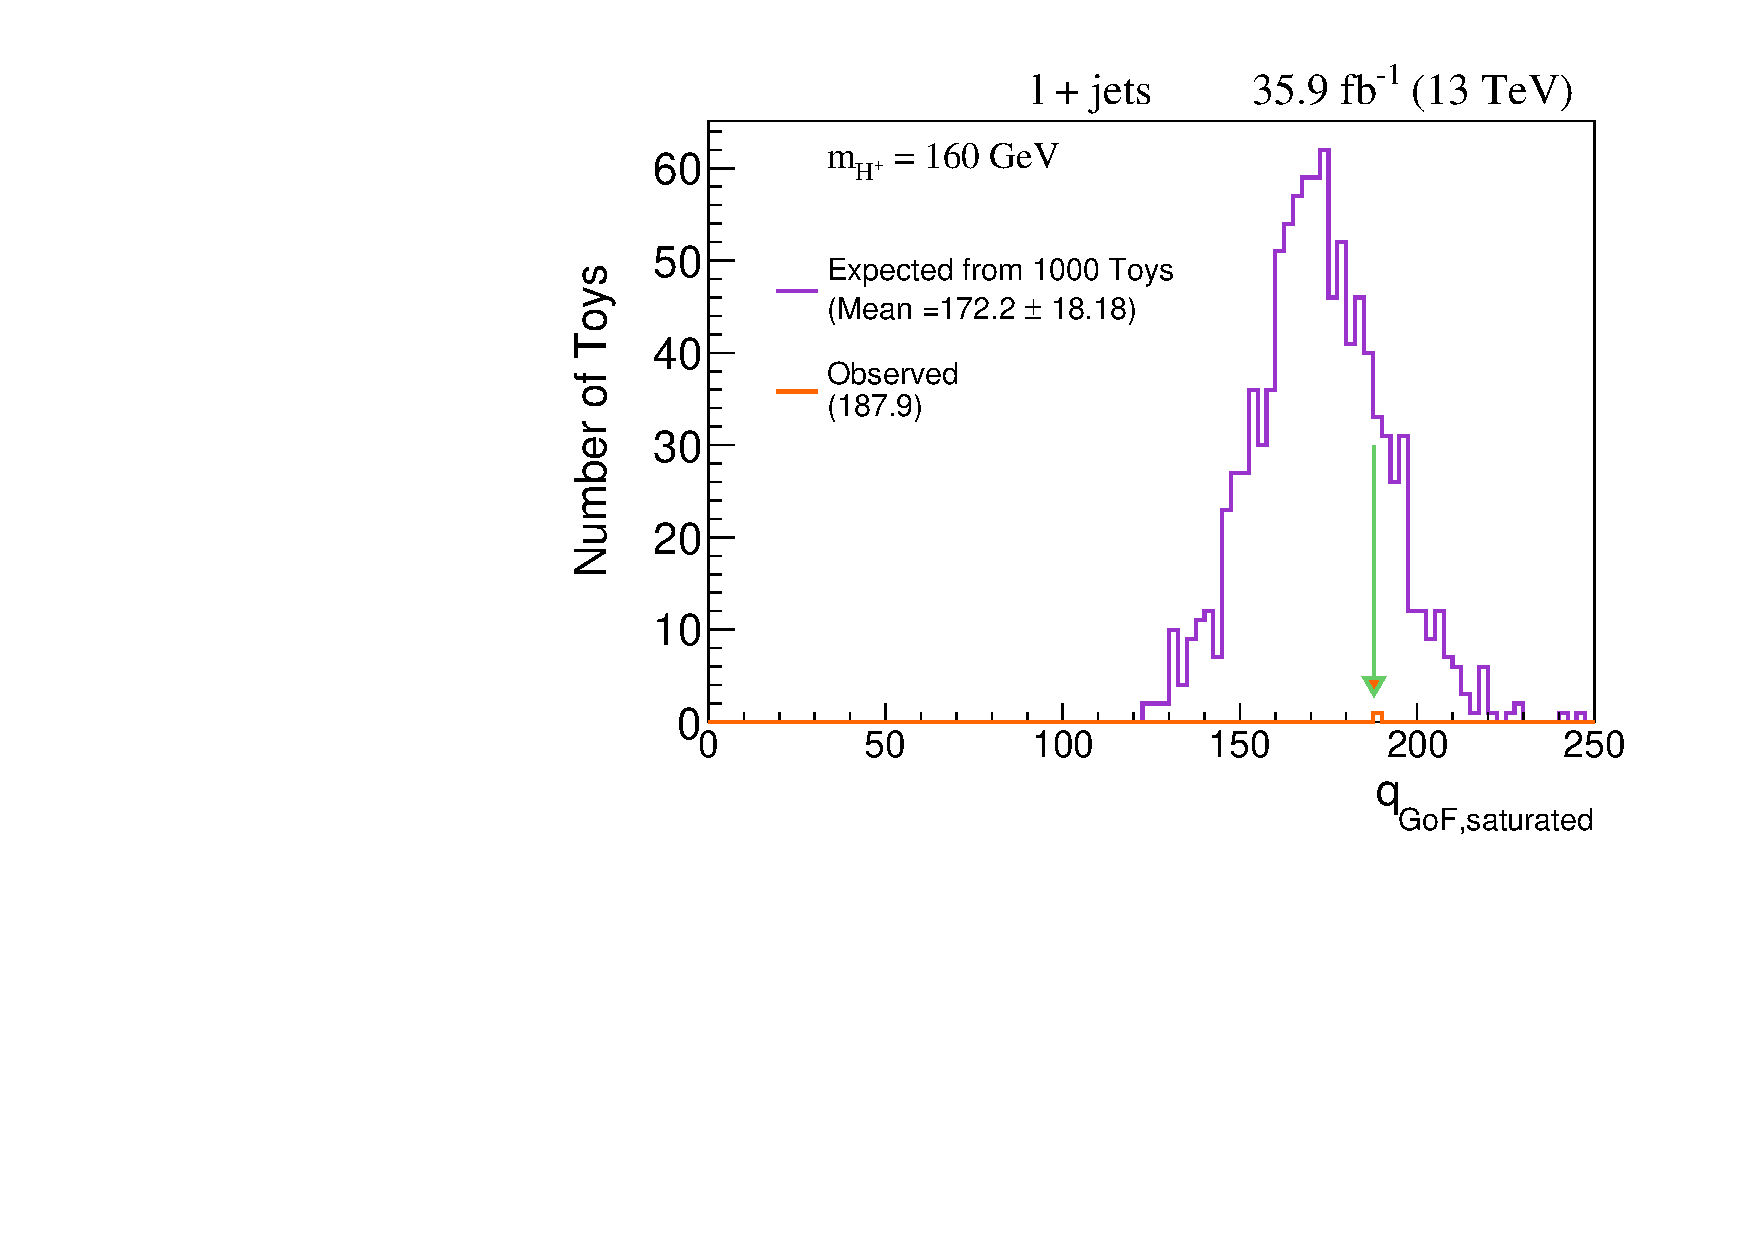
\includegraphics[width=0.40\linewidth]{Image/GOF/GOF_mu_ele_Cat3_cTagEx_160.pdf}}
    \caption{Goodness of fit for \ljets from exclusive charm categories.}
    \label{fig:GOF}
\end{figure}
\begin{table}
\caption{Goodness of fit for \mujets channel, from different event categories.}
\label{tab:gofMu}
\centering
\begin{adjustbox}{max width=\textwidth}
\begin{tabular}{ ccccccc}
\hline
\hline
\multicolumn{1}{c}{{\bf{$m_{H^\pm}$}}} & \multicolumn{2}{c}{$\mjj(Inc)$} & \multicolumn{2}{c}{$\mjj(Inc ~CTagL)$} & \multicolumn{2}{c}{$\mjj(Ex ~CTag)$} \\

(GeV) & from toys & from data & from toys & from data & from toys & from data  \\
 \hline
\hline
80  & 29.57 $\pm$ 7.284 & 49.22 & 29.34 $\pm$ 7.946 & 52.86 & 88.91 $\pm$ 13.35 & 108.9\\
  
90  & 29.39 $\pm$ 7.533 & 49.22 & 29.14 $\pm$ 7.301 & 52.86 & 88.86 $\pm$ 12.86 & 108.9\\
  
100  & 29.43 $\pm$ 7.594 & 49.22 & 29.52 $\pm$ 7.695 & 52.86 & 88.57 $\pm$ 12.87 & 108.9\\
  
120  & 29.64 $\pm$ 9.094 & 49.22 & 29.67 $\pm$ 7.547 & 52.86 & 88.11 $\pm$ 12.68 & 108.9\\
  
140  & 29.45 $\pm$ 7.441 & 49.22 & 29.89 $\pm$ 7.778 & 52.86 & 88.83 $\pm$ 13.13 & 108.9\\
  
150  & 29.66 $\pm$ 7.976 & 49.22 & 29.51 $\pm$ 7.602 & 52.86 & 88.34 $\pm$ 12.86 & 108.9\\
  
155  & 29.31 $\pm$ 7.22 & 49.22 & 29.71 $\pm$ 8.658 & 52.86 & 88.17 $\pm$ 13.02 & 108.9\\
  
160  & 29.45 $\pm$ 7.746 & 49.22 & 29.7 $\pm$ 8.043 & 52.86 & 88.38 $\pm$ 13.11 & 108.9\\
\hline
\end{tabular}
\end{adjustbox}
\end{table}

\begin{table}
\caption{Goodness of fit for \ejets channel, from different event categories.}
\label{tab:gofEle}
\centering
\begin{adjustbox}{max width=\textwidth}
\begin{tabular}{ ccccccc}
\hline
\hline
\multicolumn{1}{c}{{\bf{$m_{H^\pm}$}}} & \multicolumn{2}{c}{$\mjj(Inc)$} & \multicolumn{2}{c}{$\mjj(Inc ~CTagL)$} & \multicolumn{2}{c}{$\mjj(Ex ~CTag)$} \\

(GeV) & from toys & from data & from toys & from data & from toys & from data  \\
 \hline
\hline
80  & 29.58 $\pm$ 7.663 & 38.24 & 29.15 $\pm$ 7.537 & 37.44 & 88.16 $\pm$ 12.64 & 81.26\\
  
90  & 29.9 $\pm$ 7.966 & 36.8 & 29.21 $\pm$ 7.647 & 37.3 & 87.68 $\pm$ 12.23 & 81.26\\
  
100  & 29.24 $\pm$ 7.653 & 38.06 & 29.61 $\pm$ 7.781 & 37.44 & 87.8 $\pm$ 12.83 & 81.26\\
  
120  & 29.22 $\pm$ 7.394 & 37.15 & 29.18 $\pm$ 7.542 & 37.44 & 87.66 $\pm$ 13.02 & 81.26\\
  
140  & 29.74 $\pm$ 7.669 & 38.24 & 29.3 $\pm$ 7.607 & 37.44 & 87.68 $\pm$ 12.94 & 81.26\\
  
150  & 29.79 $\pm$ 7.717 & 38.24 & 29.43 $\pm$ 7.645 & 37.44 & 87.81 $\pm$ 12.66 & 81.26\\
  
155  & 29.31 $\pm$ 7.612 & 38.24 & 29.88 $\pm$ 8.07 & 37.44 & 88.07 $\pm$ 12.6 & 81.26\\
  
160  & 29.1 $\pm$ 7.687 & 38.24 & 29.57 $\pm$ 7.951 & 37.44 & 87.92 $\pm$ 12.51 & 81.26\\
\hline
\end{tabular}
\end{adjustbox}
\end{table}

\begin{table}
\caption{Goodness of fit for \ljets channel, from different event categories.}
\label{tab:gofLep}
\centering
\begin{adjustbox}{max width=\textwidth}
\begin{tabular}{ ccccccc}
\hline
\hline
\multicolumn{1}{c}{{\bf{$m_{H^\pm}$}}} & \multicolumn{2}{c}{$\mjj(Inc)$} & \multicolumn{2}{c}{$\mjj(Inc ~CTagL)$} & \multicolumn{2}{c}{$\mjj(Ex ~CTag)$} \\

(GeV) & from toys & from data & from toys & from data & from toys & from data  \\
 \hline
\hline
80  & 58.85 $\pm$ 10.63 & 87.27 & 58.96 $\pm$ 10.77 & 89.81 & 169.6 $\pm$ 15.31 & 187.8\\
  
90  & 58.6 $\pm$ 10.34 & 87.27 & 58.94 $\pm$ 10.44 & 89.81 & 170.2 $\pm$ 15.18 & 187.9\\
  
100  & 58.62 $\pm$ 10.75 & 87.27 & 58.84 $\pm$ 10.92 & 89.81 & 169.5 $\pm$ 14.53 & 187.9\\
  
120  & 58.97 $\pm$ 10.8 & 87.27 & 58.77 $\pm$ 10.46 & 89.81 & 170.1 $\pm$ 15.47 & 187.8\\
  
140  & 58.89 $\pm$ 10.34 & 87.27 & 58.52 $\pm$ 10.55 & 89.79 & 170.4 $\pm$ 14.99 & 187.9\\
  
150  & 58.65 $\pm$ 10.65 & 87.27 & 58.48 $\pm$ 10.34 & 89.79 & 170 $\pm$ 15.4 & 187.9\\
  
155  & 58.57 $\pm$ 10.9 & 87.27 & 58.98 $\pm$ 10.85 & 89.79 & 169.9 $\pm$ 15.45 & 187.8\\
  
160  & 58.63 $\pm$ 10.95 & 87.27 & 59.24 $\pm$ 11.97 & 89.79 & 169.7 $\pm$ 15.69 & 187.9\\
\hline
\end{tabular}
\end{adjustbox}
\end{table}



